\chapter{Introduction}\label{ch:intro}

Artificial Intelligence (AI) has advanced at a rapid rate in recent years, with generative models and tools such as ChatGPT, GitHub Copilot, and Amazon CodeWhisperer achieving rapid widespread adoption \cite{chatgpt_growth_2023}. The pervasive integration of these technologies into higher education has occurred at a speed that necessitates a fundamental re-evaluation of foundational programming pedagogy \cite{Alpizar-Chacon2025}. Although these tools offer the potential to scaffold understanding and increase learning efficiency, their unguided use threatens to undermine core educational goals, including conceptual mastery, problem-solving resilience, and academic integrity \cite{Becker}.

This presents a critical challenge for educators: how to evolve pedagogy in a world where functional code can be generated instantly from natural language prompts. Simply banning these tools is both impractical and educationally regressive, as it denies students the opportunity to learn how to use the technologies that are reshaping the software development industry. In contrast, uncritical adoption risks producing "AI-dependent" students who outsource the entire problem-solving process to a Large Language Model (LLM), in the process  bypassing the critical cognitive struggle required to achieve computational fluency \cite{Bassner2026}. Without pedagogical guardrails, students often lack the instruction necessary to use AI as a supportive tutor rather than a solution generator, leading to significant learning gaps that are often obscured until formal assessment.

Furthermore, the ability of AI to generate complete and correct code, particularly at an introductory level, has created an immediate crisis of academic integrity. Traditional assessment models, which often rely on the submission of code, are now highly vulnerable to automated cheating \cite{Lau2023}. The central task for modern computer science education is therefore not to resist AI, but to strategically and responsibly integrate it into the curriculum through interventions that preserve the value of a degree.

This thesis confronts this challenge by building and testing two specific, scalable AI-driven interventions designed to strategically integrate these technologies into the introductory programming landscape:

\begin{itemize}
    \item \textbf{A Course-Grounded AI Tutor:} Developed using Retrieval-Augmented Generation (RAG), this system provides students with pedagogical guidance strictly aligned with official course materials. This ensures that the AI acts as a mentor that supports learning processes rather than as a generator that provides direct answers.
    \item \textbf{An Automated Oral Assessment System:} This system leverages LLMs to conduct scalable, interactive "interviews." These sessions test a student’s conceptual understanding of the work they submitted to ensure that the final product reflects their own reasoning and mastery.
\end{itemize}

The effectiveness of these interventions is evaluated through a mixed methods approach. This methodology combines quantitative interaction metrics, such as system usage patterns and performance data, with qualitative student surveys to assess the impact on learning, perceived fairness, and student trust.

The study uses \textit{COMP9021: Principles of Programming} at the University of New South Wales (UNSW) as a pilot case study. As a postgraduate introductory course attracting a diverse cohort of students, many of whom are transitioning from non-computer science backgrounds, COMP9021 provides an ideal pilot environment. These students must rapidly acquire foundational skills, making them highly representative of the demographic most impacted by the shift toward AI-human collaboration in technology education.

\chapter{Background}\label{ch:literature_review}

\section{The paradoxical nature of AI in Programming Education}

The integration of AI into programming education presents a fundamental challenge. Although AI tools offer significant pedagogical benefits. By automating routine tasks such as syntax correction or boilerplate code generation, they can reduce extraneous cognitive load, allowing students to focus on core programming concepts \cite{Bettayeb2024}. AI tutors can also act as adaptive learning aids, offering personalised explanations that can be particularly valuable in situations where personalised instruction is inaccessible, such as large-scale online or distance learning environments \cite{OlumideEdwards-Fapohunda2024, Zviel-Girshin2024}.

Conversely, these same capabilities introduce profound pedagogical risks. The primary concern is the potential for students to develop an uncritical over-reliance on AI, leading to a superficial understanding of programming logic \cite{Elsayed2024}. Students may use LLMs to generate solutions without cognitively engaging in the essential process of problem-solving, debugging, and critical thinking. Furthermore, the outputs of large language models are not infallible; they can produce code that is subtly incorrect or explanations that are misleading, yet deliver them with an authoritative tone that a novice learner is ill-equipped to question \cite{Zviel-Girshin2024}. This dual nature of AI necessitates a pedagogical approach that actively cultivates critical evaluation skills alongside tool proficiency.

There exist a set of core programming pedagogical principles that underpin the goals of programming education.
TODO REWORD. Teaching programming to students can be challenging because it requires instructors to ensure students understand the foundational programming logic (Ibarra-Torres et al., \href{https://link.springer.com/article/10.1007/s40593-025-00524-3\#ref-CR30}{2024}). Foundational programming logic includes understanding algorithms, data structures, syntax, and the logical flow of code (Jonsson \& Tholander, \href{https://link.springer.com/article/10.1007/s40593-025-00524-3\#ref-CR32}{2022}). It helps students build a strong understanding of programming logic, prepares them for advanced topics, and future professional challenges. 
The development of higher-order thinking skills is important in programming education, as it advances critical thinking (Smolansky et al., \href{https://link.springer.com/article/10.1007/s40593-025-00524-3\#ref-CR84}{2023}), problem-solving (Kazemitabaar et al., \href{https://link.springer.com/article/10.1007/s40593-025-00524-3\#ref-CR34}{2023a}, \href{https://link.springer.com/article/10.1007/s40593-025-00524-3\#ref-CR35}{2023b}), and creativity (Kothari, \href{https://link.springer.com/article/10.1007/s40593-025-00524-3\#ref-CR39}{2023}).  DONE REWORD
Regardless of institution approaches to AI, these principles should be kept paramount.


\section{The Crisis of Assessment and Academic Integrity}

The capabilities of modern AI have rendered many traditional assessment methods in programming education obsolete. Recent studies confirm that models such as OpenAI's GPT-5 and Google's Gemini 3 can consistently outperform novice programmers on standard introductory assignments \cite{Qureshi2023, Huckins2025}, making it trivial for students to submit work that is not their own. This directly threatens the credibility of academic credentials, as institutions cannot reliably distinguish between student and machine-generated submissions \cite{Humble2024}.

Efforts to combat, such as AI-detection software, have proven unreliable and impractical, especially for the small functional code segments typical of introductory courses \cite{Finnie-Ansley2022}. Enforcement-based strategies that ban AI usage are not only difficult to police but also create an adversarial relationship with students. 
\textbf{// some students find that they have an incentive to cheat as they feel they are falling behind if not.  TODO}
This situation has created an urgent need to fundamentally rethink assessment design, moving away from tasks that can be easily outsourced to an AI and toward methods that evaluate a student's authentic problem-solving process, validating their understanding of material.

\section{Emerging Pedagogical Responses and Their Limitations}

In response to this crisis, two divergent philosophies are emerging. A protectionist approach advocates for designing "AI-proof" assessments, such as handwritten code, oral examinations, or complex multimodal projects that are difficult for current AI to solve independently \cite{Lau2023}. While this strategy can preserve 
the integrity of certain assessments, it is not a holistic solution.
\textbf{TODO}
1. detached from the situations in which students will use code in real world
2. temporary fix, as AI continues to advance (Moore's law), complex projects are easier to solve
3. students because more versed in how to dodge AI
it risks being a temporary fix and may fail to prepare students for a professional world where AI tools are standard.


An integrationist approach argues that AI should be integrated into both the course content and course delivery methodology. 

\textbf{TODO}
\href{https://link.springer.com/article/10.1007/s40593-025-00524-3}{Literature Review on the Integration of Generative AI in Programming Education | International Journal of Artificial Intelligence in Education | Springer Nature Link} 

The most prominent example is Harvard's CS50 course, which deployed the CS50 Duck, an AI tutor built on GPT-4 \cite{Liu2024}. As seen in figure 2.1, a custom OpenAI GPT-4 wrapper with CS50-specific contextual knowledge provided via retrieval-augmented generation (RAG) endowed students with a real-time context-aware tutor. The tutor is designed to guide students with hints rather than providing direct answers. Adoption and satisfaction rates were exceptionally high, with over 80% of students reporting the tool was frequently or always helpful.

\begin{figure}[h]
    \centering
    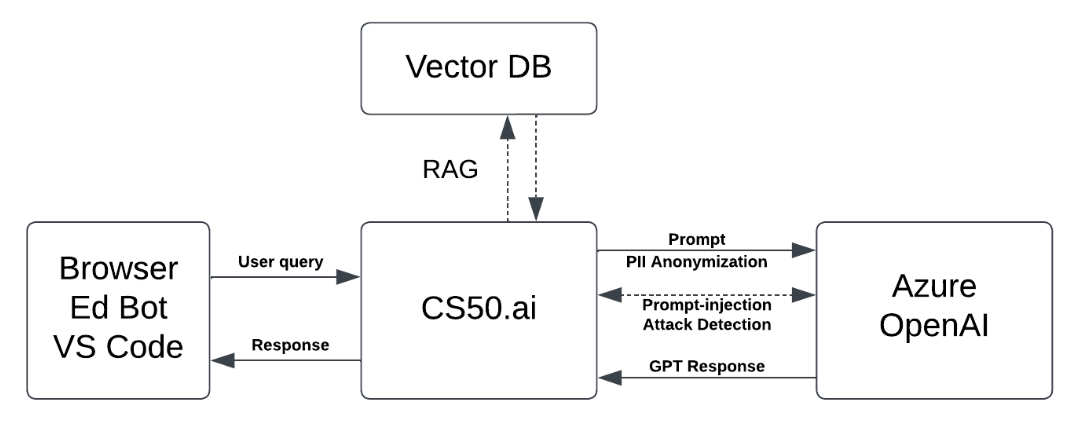
\includegraphics[width=0.8\linewidth]{Images/cs50duckArchitecture.png}
    \caption{High-level overview of the system architecture used in CS50 Duck}
    \label{fig:cs50_duck}
\end{figure}

However, the CS50 model, while successful in its context, has key limitations. There is a need to move beyond general AI assistants and investigate the efficacy of tutors that are deeply integrated with a specific course's entire ecosystem of materials, from lecture slides and textbooks to coding style guides and the history of faculty-approved answers on course forums. Such a tool could explain a difficult concept using the precise terminology of the lecturer or generate new practice problems modelled on the style of past exams, offering a truly cohesive learning experience.

\section{Developing Scalable, Authentic Assessments}

The main obstacle impeding widespread adoption of oral assessments is scalability. Conducting individual interviews is prohibitively time-consuming for instructors in large courses.

Automated feedback on code structure and functionality has proven both possible and successful, with various models capable of evaluating code quality, structure, and similarity to test cases \cite{Gambo2024, Parvathy2025}.  A representative model includes three main components, as shown in Figure 2.2:

\begin{itemize}
    \item \textbf{Syntax Error Detection Module (SEDM)}: Detects common syntax errors in code.
    \item \textbf{Structure-Based Code Assessment Model (SBCAM)}: Assesses code organization, readability, and maintainability.
    \item \textbf{Similarity and Test-Case Based Code Assessment Model (STCAM)}: Evaluates functionality through test cases and checks for code similarity to uphold academic integrity.
\end{itemize}

\begin{figure}[h]
    \centering
    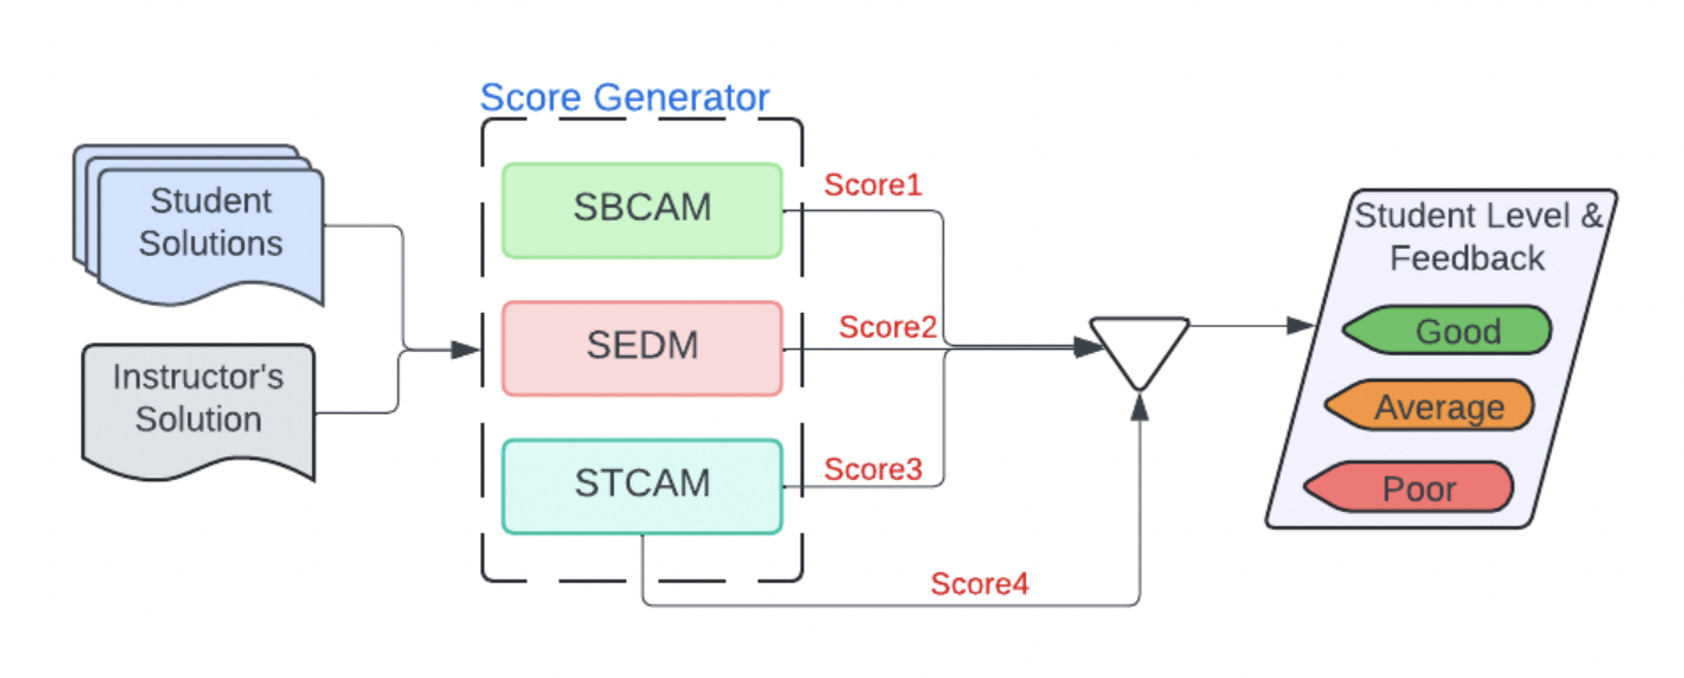
\includegraphics[width=0.7\linewidth]{Images/AutomatedFeedback.png}
    \caption{Overview of the automated code assessment system components}
    \label{fig:automated_code_assessment}
\end{figure}

These systems demonstrate that code be evaluated automatically, allowing for tailored follow-up questions to be LLM-generated to test a student's understanding. However, these models primarily assess the final product rather than the problem-solving process.

More recently, intelligent agents have been developed to automate industry-style technical interviews, using metrics such as BLEU and BERTScore to evaluate candidate responses \cite{Joseph2024}. These tools are already widespread in industry, with platforms like HireVue conducting entry-level role interviews across various sectors and evaluating candidates' technical understanding. However, these industry-focused agents are not designed for a pedagogical context. They lack the framework to assess a student's understanding of their own previously completed work or to probe for conceptual knowledge related to a course curriculum. 

\section{AI solutions for education }

TODO add context about how this is useful for AI tools in an educational context

\subsubsection{Retrieval Augmented Generation (RAG)}
RAG combines a large language model (LLM) with an external knowledge source to improve accuracy, reduce hallucinations, and enable domain-specific responses \cite{Lewis2021}. In this approach, relevant documents are retrieved from a structured knowledge base or vector store and provided to the model as additional context during generation. This allows the system to incorporate information beyond the model’s static training data, delivering more accurate and contextually relevant outputs \cite{Min2022}. RAG has a wide range of applications. It can be used to perform real-time searches over institution documentation, policies, or technical repositories, enabling instant access to relevant information. Figure \ref{fig:aws_rag} displays a potential implementation of RAG.

\begin{figure}[h]
    \centering
    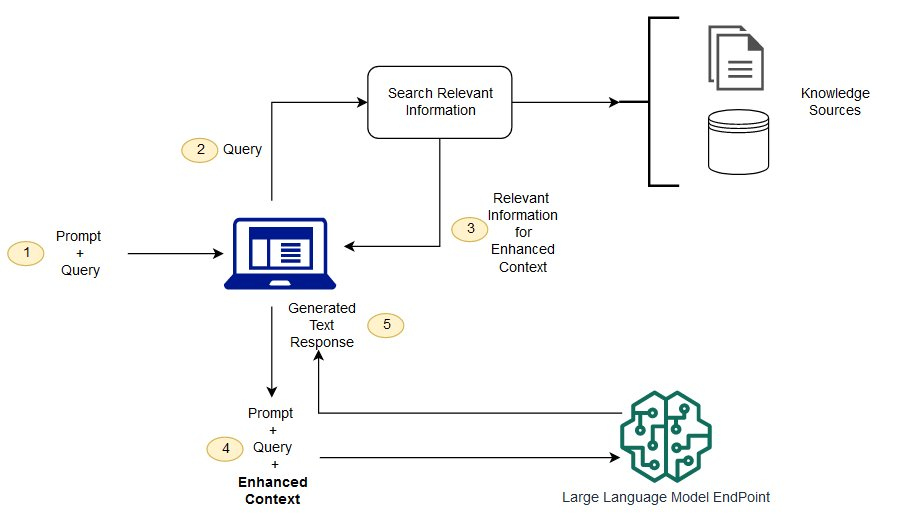
\includegraphics[width=0.85\linewidth]{Images/awsRag.jpg}
    \caption{High-level architecture of Retrieval-Augmented Generation (RAG)}
    \label{fig:aws_rag}
\end{figure}


However, retrieval adds extra processing steps, which can increase latency and overall system complexity. In addition, the indexing pipelines, embeddings, and vector databases that underpin RAG must be maintained continuously. As a result, without regular maintenance, the quality and relevance of the retrieved information can degrade over time.

\subsubsection{Model Context Protocol (MCP) Servers}

MCP servers provide a standardised framework for managing and delivering context to large language models (LLMs). They act as middleware between the AI model and its information sources, packaging relevant course content, user data, and system instructions into a structured format \cite{Hou2025}. This enables consistent, context-aware interactions across different AI components, and ensures that all systems are grounded in the same authoritative data. MCP can facilitate multi-step workflows by chaining together different tools, enabling secure collaboration between systems and agents by allowing them to access and share information efficiently  \cite{Ahmadi2025}. A sample implementation of an MCP server is shown in figure \ref{fig:mcp_architecture}.

\begin{figure}[h]
    \centering
    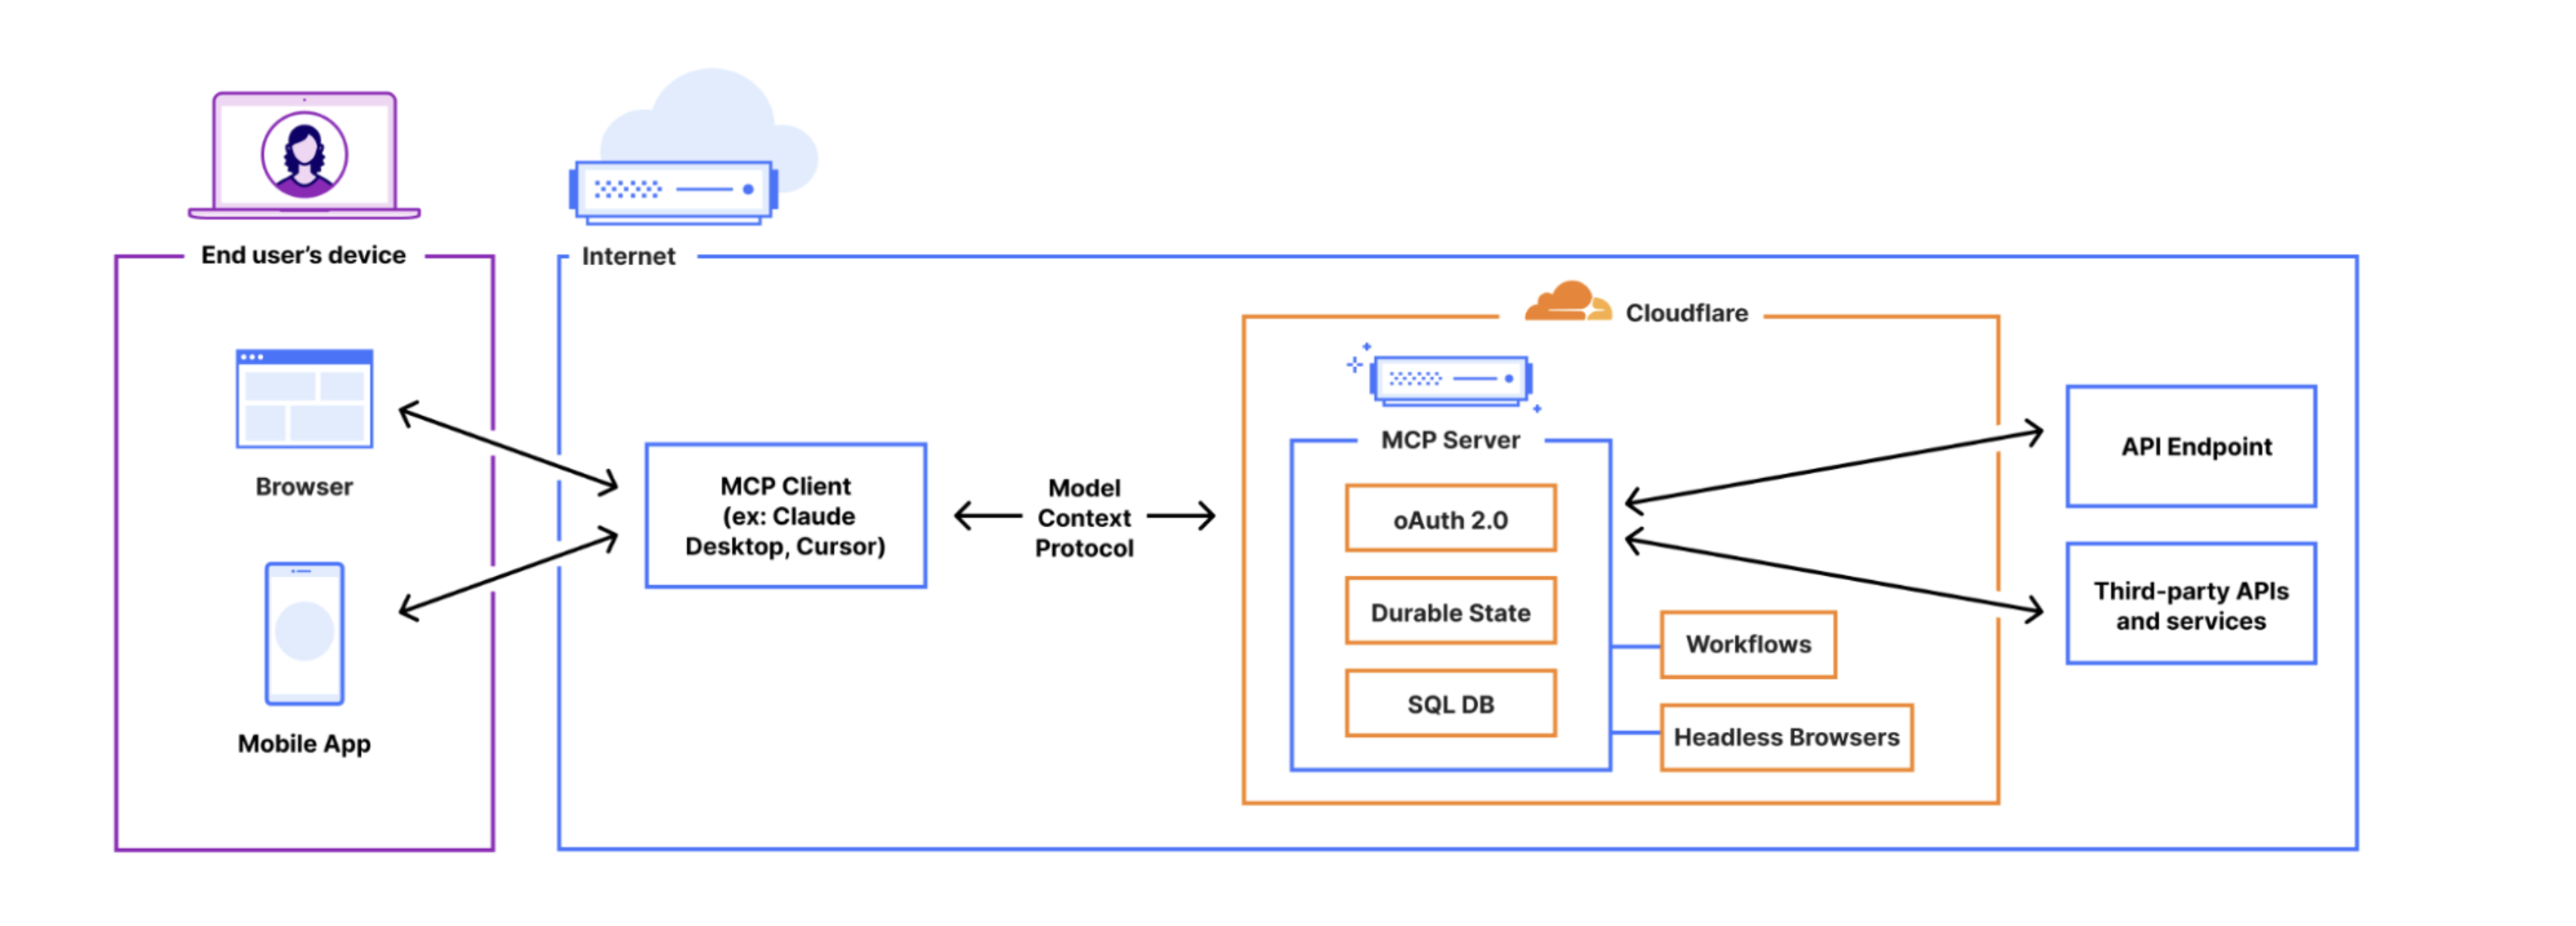
\includegraphics[width=1.1\linewidth]{Images/mcp.png}
    \caption{Example architecture for an authenticated MCP server connecting multiple AI components with shared context.}
    \label{fig:mcp_architecture}
\end{figure}

However, the MCP integration process is complex, which may result in increased operational costs depending on deployment scale and infrastructure choices. Additionally, the performance of the tool degrades rapidly as the number of external integrations increases.

\chapter{Research Questions} \label{ch:research_questions}

Building on the pedagogical tensions and opportunities outlined in the literature review, this chapter defines the specific research gaps and articulates the central problem addressed in this thesis. The preceding literature review has identified two critical, interconnected gaps in the current research on AI in programming education:

\section{Gaps in Current Research}

Lack of Deeply-Grounded AI Tutors: While general AI assistants show promise, there is a lack of research on tutors that are deeply grounded in a comprehensive corpus of course-specific materials, including lecture slides, textbooks, past exam questions, coding style guides, and validated forum discussions. It is unknown if this deep, holistic grounding provides a significant pedagogical advantage over more generic tools. TODO refine. figure out how this is unique

Absence of a Scalable, Pedagogical Oral Assessment Model: Traditional assessments are vulnerable to AI misuse. Oral examinations are a robust alternative but are not scalable. The specific need is for a system that can automate this process in an educationally relevant way, focusing on having students verbally justify their own submitted code and answer related conceptual questions, a model distinct from industry-oriented live coding interviews.

TODO reframe
By combining automated code analysis with intelligent interview agents, it would be possible to develop a scalable framework for automated oral assessments, retaining the pedagogical benefits of live interviews while making them feasible in large-scale programming courses.

What is needed is a system that can conduct a structured, one-on-one dialogue with a student, asking them to explain their submitted code and answer related conceptual questions, effectively shifting the assessment focus from "what did you produce?" to "how do you think?" 

\section{Problem Statement}

The literature review leads to the following problem statement:

"How can AI tools be strategically and responsibly integrated into introductory programming courses to enhance learning outcomes, preserve core educational values, and align with emerging industry norms, using UNSW’s COMP9021 as a case study example?"

This thesis addresses the following research questions:

1. To what extent does a course-grounded AI tutor built on course specific materials improve students’ conceptual understanding and learning experience compared to general-purpose AI tools?

2. Can a scalable AI-driven oral assessment system effectively evaluate a student’s programming competency by probing their reasoning and understanding of their own code, and does it strengthen academic integrity compared to traditional assessments?

3. How do students perceive the usefulness, fairness, and trustworthiness of AI-based tutoring and assessment systems in a foundational programming course?

To answer these questions, this study will design, deploy, and evaluate these two distinct AI interventions within UNSW’s COMP9021, providing an empirical basis for a new model of AI-augmented programming pedagogy.


\chapter{Methodology} \label{ch:preliminary_work}

\section{Project-Dependant Skills}

TODO talk past tense
Having established the research problem, this chapter details the groundwork required for the technical and ethical implementation of the proposed systems. This section will detail the techniques and knowledge necessary for a successful implementation of the project. 

Overview - build, trial and evaluate systems within pilot course at unsw. From feb - april 2026 (unsw trimester 1). full rollout of AI tutor. limited voluntary trial of oral assessments to 1. check efficacy and 2. gather feedback to address and trial ethical, privacy and fairness concerns

\section{Software Development Methodology}

The project will adopt an agile-inspired development methodology, emphasising iterative prototyping, continuous evaluation. this research will form the basis for further experimentation and development. Agile methods are particularly well-suited due to their adaptability to evolving requirements, user feedback, and emerging technological capabilities \cite{KentBeck2001, DeLucia2010}.

Recognising that this is a living project impacting students education, quality and continuity is important. prioritised

\begin{itemize}
    \item \textbf{solid and thorough testing:} Unit tests, integration tests, and regression tests will be incorporated into the CI/CD pipeline to ensure functional correctness and prevent the reintroduction of bugs.
    \item \textbf{Performance Monitoring and Logging:} Application metrics and AI inference performance will be monitored in real time, with logs stored securely for audit and troubleshooting purposes.
    \item \textbf{Documentation and Knowledge Management:} Technical documentation will be maintained in parallel with development, covering architecture diagrams, API specifications, and operational guides to ensure maintainability.
    - anything else relevant
\end{itemize}

\section{Project Ethical Considerations}

The project will follow UNSW’s \textit{Human Research Ethics Guidelines} \cite{UNSW2025} and the \textit{Australian National Statement on Ethical Conduct in Human Research}, ensuring AI tools in education are deployed fairly, transparently, and securely.

\textbf{Data Privacy and Security} — All student data will be stored securely in compliance with the Australian Privacy Principles under the \textit{Privacy Act 1988}. Access will be restricted to authorised personnel, and retention will follow UNSW’s records management policy.

\textbf{Informed Consent} — Participation in trials will be voluntary, with clear explanations of the project’s purpose, data use, and the right to withdraw.

\textbf{Transparency} — Feedback and grading decisions will be traceable, with tutors able to review rationale and transcripts, with explanations made available to students on request.

\textbf{Ethics Approval} — The project will obtain UNSW Human Research Ethics Committee (HREC) approval before deployment.

\section{Initial Product Design}

\subsection{Personal AI tutor}

\subsubsection{Architecture Decisions}

Figure~\ref{fig:tutor_arch} presents a high-level design in which a Model Context Protocol (MCP) server manages all interactions between the LLM and course resources. The MCP layer standardises context packaging (course materials, user/session state, system prompts) and mediates calls to external tools, enabling the tutor to answer student queries with grounded, auditable responses.

AWS services are a solid candidate to  streamline security, observability, and scale. In this configuration, MCP endpoints are hosted behind an API gateway with serverless compute for tool adapters. Storage and search services back the retrieval flow, permissioned behind AWS Cognito.

A dedicated data-ingestion pipeline keeps the knowledge base updated. Course resources (lecture slides, specs, forum FAQs, exemplar solutions, policy documents) are uploaded, transformed and indexted into a vector store for later retrieval and search. Updates (e.g., new forum posts or amended specs) trigger re-indexing jobs so that retrieval remains consistent with the latest materials.

This architecture isolates capabilities behind MCP tools, simplifies policy enforcement (what the AI tutor is allowed to access and say), and supports easy future extension.


\begin{figure}[H]
    \centering
    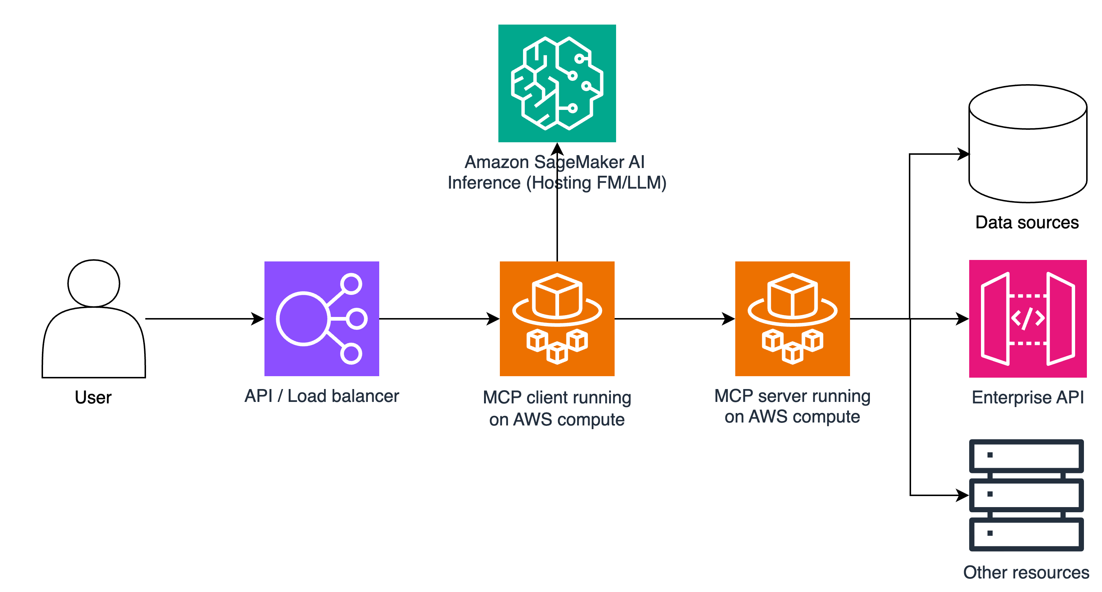
\includegraphics[width=0.8\linewidth]{Images/mcparchitecture.png}
    \caption{Potential architecture diagram for AI tutor using MCP}
    \label{fig:tutor_arch}
\end{figure}
\FloatBarrier


\subsubsection{User Stories and Acceptance Criteria}

\textbf{User Story 1: Context-Aware Question Answering}\\
As a COMP9021 student, I want to ask the AI tutor questions about course content and get answers grounded in official materials, so that I receive accurate, relevant, and up-to-date explanations.  
\emph{Acceptance Criteria:}
\begin{itemize}
    \item Retrieves and references relevant sections of course materials.
    \item Responses are factually correct according to the latest course version.
    \item Cites sources or points to relevant lecture slides or problem sets.
\end{itemize}

\textbf{User Story 2: Code Review and Feedback}\\
As a student, I want the AI tutor to review my Python code and give feedback on logic, structure, and style, so that I can improve code quality before submission.  
\emph{Acceptance Criteria:}
\begin{itemize}
    \item Identifies syntax errors, logical issues, and poor coding practices.
    \item Feedback aligns with COMP9021 coding style guidelines.
    \item Offers at least one alternative solution or improvement.
\end{itemize}

\textbf{User Story 3: Practice Question Generation}\\
As a student, I want the AI tutor to generate practice questions tailored to my weak areas, so that I can focus my study more effectively.  
\emph{Acceptance Criteria:}
\begin{itemize}
    \item Uses quiz/assignment performance to identify weak areas.
    \item Matches difficulty to course assessment standards.
    \item Provides model solutions and explanations.
\end{itemize}

\textbf{User Story 4: Step-by-Step Problem Solving Guidance}\\
As a student, I want the AI tutor to guide me step-by-step through problem-solving, so that I can understand the reasoning process, not just the final answer.  
\emph{Acceptance Criteria:}
\begin{itemize}
    \item Breaks problems into logical, manageable steps.
    \item Explains the purpose of each step.
    \item Waits for student input before revealing the next step.
\end{itemize}

\textbf{User Story 5: Personalised Study Plan}\\
As a student, I want the AI tutor to create a personalised weekly study plan, so that I stay on track with course deadlines and revision.  
\emph{Acceptance Criteria:}
\begin{itemize}
    \item Includes lecture review, practice, and revision time.
    \item Syncs deadlines with COMP9021 assessment schedule.
    \item Updates automatically based on progress.
\end{itemize}

\begin{table}[H]
\centering
\caption{Summary of User Stories for Personal AI Tutor}
\label{tab:userstories_tutor}
\renewcommand{\arraystretch}{1.2}
\begin{tabular}{p{0.8cm} p{6cm} p{6cm}}
\toprule
\textbf{\#} & \textbf{User Story} & \textbf{Acceptance Criteria (Summary)} \\
\midrule
1 & Personalised code feedback & Provides targeted, context-aware suggestions on student code; feedback is constructive and timely. \\
2 & Hints without full solutions & Offers progressive, hint-based guidance; avoids giving complete solutions unless explicitly requested. \\
3 & Course content integration & Uses COMP9021 materials in responses; ensures contextual relevance and accuracy. \\
4 & Error detection and explanation & Identifies syntax and logical errors; provides clear explanations with examples. \\
5 & Progress tracking & Monitors student performance; suggests topics for improvement and revision. \\
\bottomrule
\end{tabular}
\end{table}
\FloatBarrier

\subsection{Automated Oral Assessment System}

\subsubsection{Architecture Decisions}

Diagram~\ref{fig:oral_arch} represents a high-level overview of a potential implementation of the system. The end user inputs from a student are simply their assessment code submission and an oral examination. For teaching staff, they would need only to provide course teaching materials and sample solutions to the assessment.

\begin{figure}[H]
    \centering
    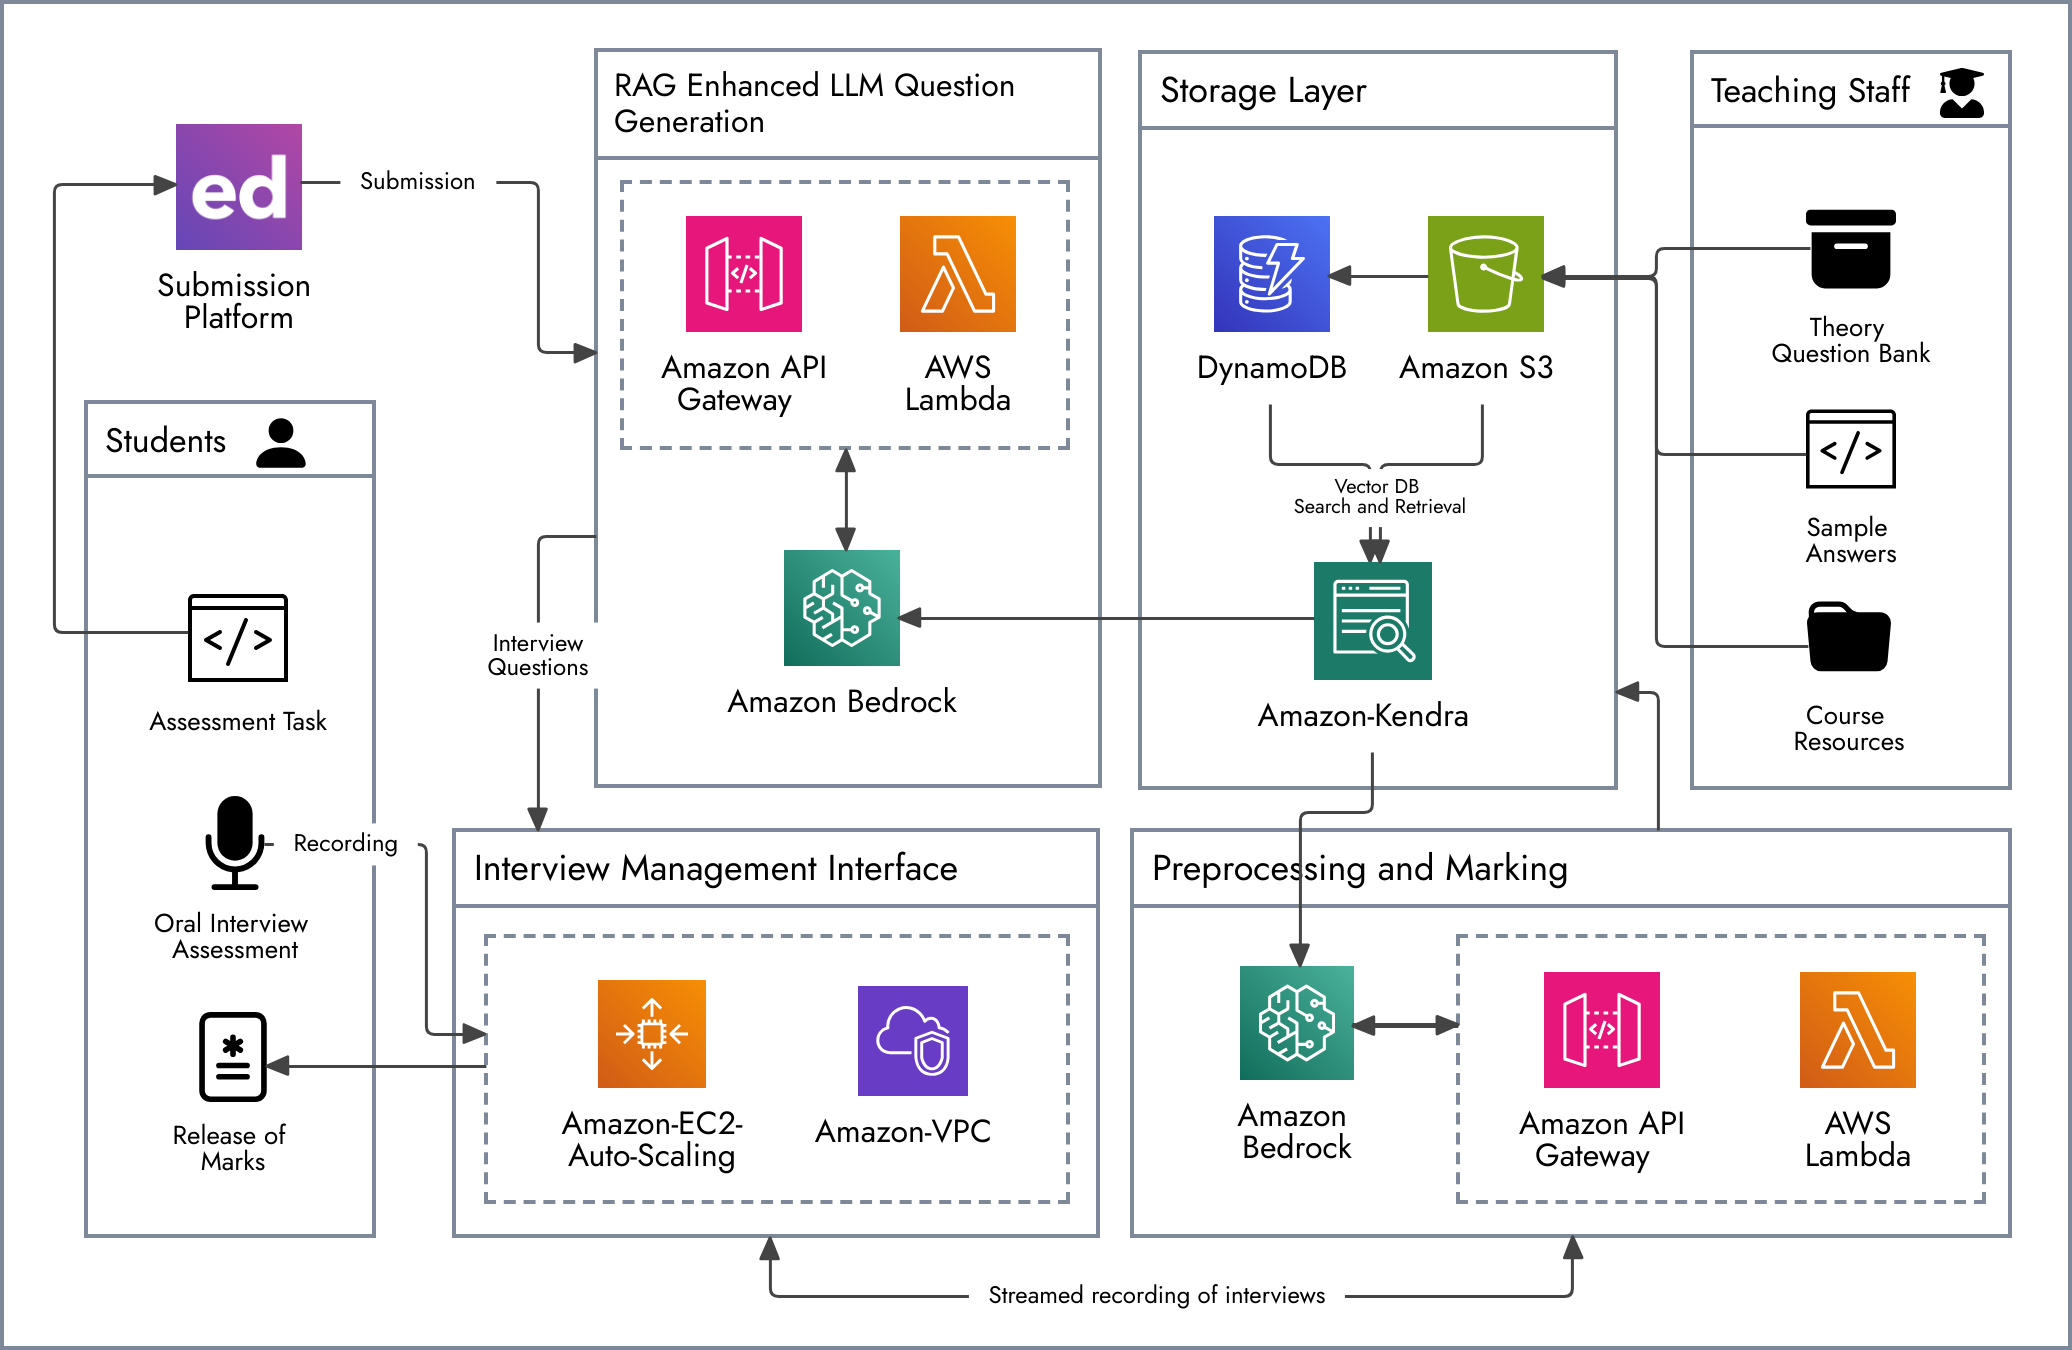
\includegraphics[width=1\linewidth]{Images/Diagram1.png}
    \caption{Potential architecture diagram for AI interviewer system}
    \label{fig:oral_arch}
\end{figure}
\FloatBarrier

\subsubsection{User Stories and Acceptance Criteria}

\textbf{User Story 1: Real-Time Oral Code Explanation}  
As a COMP9021 student, I want to be asked to explain my code during an automated interview, so that I can demonstrate my understanding of how it works.  
\textit{Acceptance Criteria:}
\begin{itemize}
    \item The system selects code segments from my submission.
    \item The system prompts me with targeted, open-ended questions.
    \item My spoken responses are recorded and transcribed accurately.
\end{itemize}

\textbf{User Story 2: Adaptive Questioning Based on Responses}  
As a COMP9021 student, I want the system to adapt its questions based on my answers, so that the interview reflects my actual understanding.  
\textit{Acceptance Criteria:}
\begin{itemize}
    \item Follow-up questions are contextually relevant to my last response.
    \item The difficulty of questions adjusts dynamically.
    \item The interview maintains an appropriate length and depth.
\end{itemize}

\textbf{User Story 3: Objective Scoring and Feedback}  
As a COMP9021 student, I want my oral responses to be scored consistently and objectively, so that I can trust the assessment process.  
\textit{Acceptance Criteria:}
\begin{itemize}
    \item The scoring system uses predefined rubrics aligned with course learning outcomes.
    \item Feedback highlights both strengths and areas for improvement.
    \item Scores are reviewed for consistency across multiple interviews.
\end{itemize}

\textbf{User Story 4: Bias-Aware Evaluation}  
As a COMP9021 student, I want the automated grading to minimise bias, so that my results are not affected by language background or accent.  
\textit{Acceptance Criteria:}
\begin{itemize}
    \item The system uses bias-mitigation techniques in evaluation.
    \item Performance is evaluated on content rather than speech fluency.
    \item A manual review option is available for disputed results.
\end{itemize}

\textbf{User Story 5: Integration with Course Assessment Systems}  
As a COMP9021 student, I want my interview results to integrate with the course’s existing assessment platform, so that I have a single place to view all my grades.  
\textit{Acceptance Criteria:}
\begin{itemize}
    \item Scores and feedback are automatically uploaded to the LMS.
    \item Results are tagged with the relevant assessment identifier.
    \item The system maintains secure handling of all assessment data.
\end{itemize}

\begin{table}[h]
\centering
\caption{Summary of User Stories for Automated Oral Assessment}
\label{tab:userstories_oral}
\renewcommand{\arraystretch}{1.2}
\begin{tabular}{p{0.8cm} p{6cm} p{6cm}}
\toprule
\textbf{\#} & \textbf{User Story} & \textbf{Acceptance Criteria (Summary)} \\
\midrule
1 & Real-time oral code explanation & Selects code segments; asks open-ended questions; records and transcribes accurately. \\
2 & Adaptive questioning & Adjusts difficulty and relevance of questions dynamically based on responses. \\
3 & Objective scoring and feedback & Uses predefined rubrics; ensures consistency; provides constructive feedback. \\
4 & Bias-aware evaluation & Minimises bias related to language or accent; allows manual review if needed. \\
5 & LMS integration & Automatically uploads results to LMS; maintains secure handling of assessment data. \\
\bottomrule
\end{tabular}
\end{table}

\section{Project Evaluation Plan}

To measure the effectiveness and impact of the developed systems, a structured evaluation process will be conducted during the deployment phase. The primary method of data collection will be a questionnaire distributed to students enrolled in COMP9021 during the trial period. The questionnaire is designed to capture both quantitative and qualitative feedback on usability, perceived learning benefits, and the overall experience of interacting with the AI Tutor and Automated Oral Assessment systems.

The evaluation will focus on:
\begin{itemize}
    \item Assessing improvements in learning outcomes and conceptual understanding.
    \item Measuring usability, accessibility, and satisfaction with the systems.
    \item Identifying potential challenges, limitations, and unintended consequences.
    \item Comparing student experiences between AI-assisted learning and traditional assessment methods.
\end{itemize}

\subsection*{Proposed Questionnaire}

The questionnaire will combine Likert-scale questions, multiple-choice questions, and open-ended responses to provide both measurable and descriptive insights.

\subsection{Part 1: AI Tutor Evaluation}
\begin{enumerate}
    \item How frequently did you use the AI Tutor during the course? (Never / Rarely / Sometimes / Often / Very often)
    \item How helpful did you find the AI Tutor in understanding course concepts? (1 = Not helpful, 5 = Extremely helpful)
    \item Did the AI Tutor improve your ability to solve problems independently? (Yes / No / Unsure)
    \item Rate the clarity and accuracy of explanations provided by the AI Tutor. (1–5 scale)
    \item What was the most useful feature of the AI Tutor? (Open-ended)
    \item What improvements would you suggest for the AI Tutor? (Open-ended)
\end{enumerate}

\subsection{Part 2: Automated Oral Assessment Evaluation}

\begin{enumerate}
    \item How confident were you in explaining your code and reasoning during the oral assessment? (1–5 scale)
    \item Did the oral assessment format help you better understand your own work? (Yes / No / Unsure)
    \item How fair and accurate did you find the automated evaluation of your responses? (1–5 scale)
    \item Did the oral assessment highlight areas for improvement that you were previously unaware of? (Yes / No)
    \item What aspects of the oral assessment were most beneficial? (Open-ended)
    \item What changes would make the oral assessment more effective? (Open-ended)
\end{enumerate}

\subsection{Part 3: Comparative and Overall Impact}
\begin{enumerate}
    \item Compared to traditional assessments, how effective were these tools in supporting your learning? (1–5 scale)
    \item Which assessment method do you feel best demonstrated your understanding of the course material? (Multiple choice: AI Tutor tasks / Oral assessment / Traditional assignments / Mixed approach)
    \item Do you believe these tools should be used in future course offerings? (Yes / No / Unsure)
    \item Additional comments on your overall experience. (Open-ended)
\end{enumerate}

\begin{table}[h]
\centering
\caption{Mapping of questionnaire questions to project evaluation goals}
\label{tab:eval_mapping}
\renewcommand{\arraystretch}{1.4} % Increases row height for readability
\begin{tabular}{p{5cm} p{9cm}}
\toprule
\textbf{Project Goal} & \textbf{Related Questionnaire Questions} \\
\midrule
Assess improvements in learning outcomes &
Part 1: Q2, Q3, Q4; Part 2: Q2, Q4; Part 3: Q1, Q2 \\[4pt]

Measure usability and satisfaction &
Part 1: Q1, Q2, Q4, Q5, Q6; Part 2: Q1, Q3, Q5, Q6; Part 3: Q3 \\[4pt]

Identify potential limitations &
Part 1: Q6; Part 2: Q6; Part 3: Q4 \\[4pt]

Compare experiences between AI-assisted and traditional learning &
Part 3: Q1, Q2, Q3 \\
\bottomrule
\end{tabular}
\end{table}

The collected data will be analysed using both statistical methods (for quantitative questions) and thematic coding (for qualitative responses) to generate a comprehensive evaluation of system performance and student reception.

\chapter{Results}

\chapter{Conclusions}  \label{ch:conclusions}
This initial report has established the background, motivation, and preliminary design for investigating the integration of AI tools into introductory programming education, using COMP9021 as a pilot context. The literature review identified both the opportunities—such as personalisation, improved feedback, and enhanced accessibility—and the challenges, including risks to academic integrity, over-reliance, and bias.

Preliminary planning has outlined two core applications for development: a course-specific AI tutor and an automated oral assessment framework. Technical options, such as the use of Retrieval-Augmented Generation (RAG) and Model Context Protocol (MCP) servers, have been explored to support these systems. A project methodology, ethical considerations, and an evaluation framework have also been defined.

The next stage of work will focus on prototype development, integration into the COMP9021 teaching environment, and structured evaluation with students. Findings from these stages will guide refinements and inform recommendations for responsible AI adoption in programming education.

\nocite{*}